\chapter{IMPLEMENTAÇÃO DAS TÉCNICAS}\label{ch:implementacao}

Este capítulo tem como finalidade apresentar, com um maior nível de detalhamento, as técnicas utilizadas neste trabalho, com o objetivo de atingir as metas propostas na seção~\ref{sec:objetivos}.

\section{COLETA DE DADOS}
Uma característica comentada anteriormente sobre a rede social \textit{Twitter} é a disponibilidade de informações de eventos em tempo real. Os \textit{tweets} podem ser postados com o intuito de comentar sobre a final de um campeonato de futebol, datas importantes, acontecimentos internacionais e políticos, entre outros.

Para este trabalho foi aproveitado o dia 17 de abril de 2016, onde foi realizado a votação no Congresso Brasileiro pela continuação do processo de Impeachment do cargo de presidente da senhora Dilma Rousseff. Neste dia, milhares de \textit{tweets} foram publicados utilizando a \textit{hashtag} \#ImpeachmentDay, a fim de comentar sobre o evento e, também, a atual situação política do Brasil.

Com a finalidade de coletar todos os dados da referida \textit{hashtag}, foi desenvolvido um \textit{script} que utiliza o serviço da API de \textit{streaming} do \textit{Twitter}.

As primeiras linhas mostradas no Código~\ref{coleta-script} servem para importar as bibliotecas e objetos necessários para a utilização da API do \textit{Twitter}, assim como as informações das chaves de acesso e \textit{tokens} para o protocolo OAuth, que são fundamentais para a comunicação com o serviço de \textit{Stream}.

\lstinputlisting[language=Python, label=coleta-script, caption=\textit{Script} coletar-hashtags.py]{Cap5/src/coletar-hashtags.py}

Destaca-se neste código que a partir da linha 11 é criado uma classe que instancia um serviço de escuta para este \textit{Stream}. O serviço de escuta é responsável por observar todos os \textit{tweets} que são publicados e, após identificar no \textit{tweet} alguma palavra ou a \textit{hashtag} semelhante às palavras declaradas na linha 28, captura e imprime na tela de execução do \textit{script}.

Quando este \textit{script} está em execução é mostrado na tela todos os \textit{tweets}, já filtrados, que estão sendo coletados. Porém, estes não estão persistindo em nenhum arquivo ou banco de dados. Com o intuito de salvar todos estes dados, foi utilizado o comando \textit{stdout} ($>$), que está presente em sistemas operacionais de base \textit{Unix}. Este comando permite redirecionar a saída do código anterior, no caso a execução do \textit{script} coletar-hashtags.py, para um novo arquivo ou um arquivo já existente, conforme ilustrado pela Figura~\ref{exec-coleta}.

\begin{figure}[h]
	\centering
	\fbox{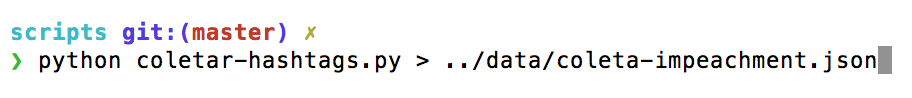
\includegraphics[width=0.95\textwidth]{Cap5/imagens/execucao-script}}
    \vspace{0.1cm}
	\caption{Execução do \textit{script} para coleta de dados}
	\fonte{Elaborado pelo autor}
	\label{exec-coleta}
\end{figure}

O \textit{script} apresentado no Código~\ref{coleta-script} permaneceu em execução durante 12 horas (das 10:30 às 22:30) do dia 17 de abril, resultando em um arquivo de 2.6 gigabytes. O formato deste arquivo é um JSON, onde apresenta todas as informações presentes em um \textit{tweet}, como demonstrado através do Código~\ref{peda-json}.

\lstinputlisting[language=Python, label=peda-json, caption=Exemplo de um \textit{tweet} no formato JSON]{Cap5/src/peda.json}

Os \textit{tweets} coletados, mediante a execução do \textit{script} apresentado no Código~\ref{coleta-script}, foram redirecionados para o arquivo \textit{coleta-impeachment.json}. Este, foi gerado através do comando \textit{stdout}, conforme ilustrado, previamente, pela Figura~\ref{exec-coleta} possibilitando a conclusão da etapa de obtenção de dados.

% Análise de Dados
\section{ANÁLISE DE DADOS}
Após a coleta dos dados foi gerado, então, um arquivo JSON de 2.6 gigabytes. Baseando-se nele, a etapa seguinte foi de analisar estes dados para extrair as informações consideradas úteis.

Foram realizados testes no arquivo JSON para verificar se existia algum tipo de \textit{dirty data}, que são informações quebradas, dados irrelevantes ou códigos que impedem a execução de \textit{scripts} de mineração \cite{dirty-data}. O único \textit{dirty data} encontrado apresenta informações referentes ao limite da API de \textit{streaming} que possui o padrão \textit{"limit":} seguido de outras informações adicionais \cite{twitter-doc}. A Figura~\ref{fig-dirty} demonstra o único padrão de \textit{dirty data} encontrado dentro do arquivo.

\begin{figure}[h]
	\centering
	\fbox{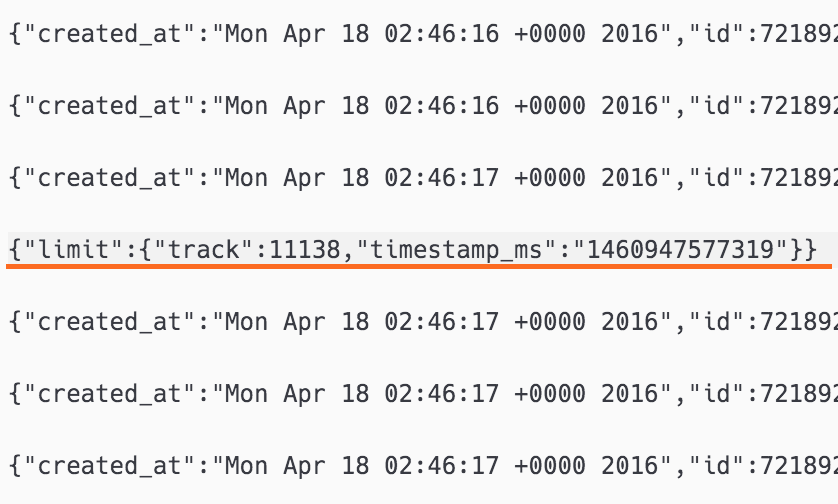
\includegraphics[width=0.95\textwidth]{Cap5/imagens/limit}}
	\vspace{0.1cm}
	\caption{\textit{Dirty Data} presente no arquivo coletado}
	\fonte{Elaborado pelo autor}
	\label{fig-dirty}
\end{figure}

Dentro das milhares linhas do arquivo, existiam algumas linhas contendo este mesmo padrão (\textit{"limit":}), que foram removidos utilizando outra ferramenta de sistemas baseados em Unix, o \textit{grep}.

A funcionalidade \textit{grep} é considerada um "canivete suíço" \space para o uso de expressões regulares e possui uma funcionalidade que permite realizar uma consulta inversa, ou seja, o usuário passa um padrão ou uma palavra que deseja encontrar dentro de um determinado arquivo e, após encontrar todas as ocorrências, o \textit{grep} seleciona tudo o que não contém este padrão ou palavra.

Logo, foi possível utilizar a consulta inversa de \textit{grep} para gerar um arquivo sem \textit{dirty data}, apenas informando o padrão \textit{"limit":} combinado com o comando de \textit{stdout} ($>$). Todos os \textit{tweets} que não apresentaram esse padrão foram redirecionados para um novo arquivo, chamado de \textit{small-data.json}, conforme apresenta a Figura~\ref{limpa-dado}.

\begin{figure}[h]
	\centering
	\fbox{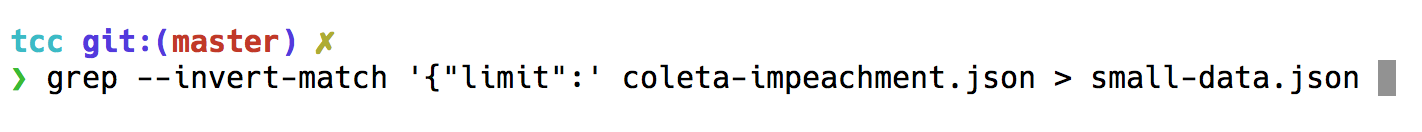
\includegraphics[width=0.95\textwidth]{Cap5/imagens/grep}}
	\vspace{0.1cm}
	\caption{Utilizando o comando \textit{grep} para gerar um novo arquivo sem \textit{dirty data}}
	\fonte{Elaborado pelo autor}
	\label{limpa-dado}
\end{figure}

Após obter o arquivo JSON, sem a presença de \textit{dirty data}, foi possível iniciar o processo de extração de conhecimento utilizando o interpretador \textit{IPython}.

Nesta primeira etapa foram importadas as bibliotecas necessárias para se trabalhar com arquivos do tipo JSON e, também, informado ao interpretador \textit{IPython} para apresentar gráficos em sua funcionalidade de \textit{notebook}, conforme a primeira linha do Código~\ref{imp-py}.

Os comandos de importação, apresentados no Código~\ref{imp-py}, foram diferenciados por sua precisão, uma vez que entre as linhas 3 e 15 carregaram-se todas as funcionalidades de cada biblioteca, enquanto a partir da linha 17, houve uma especificação na importação de funcionalidades nestas bibliotecas, permitindo o uso desta aplicação através do nome importado.


\lstinputlisting[language=Python, label=imp-py, caption=Importação de bibliotecas Python]{Cap5/src/import.py}

A primeira linha do Código~\ref{ini-py} atribuiu a variável, "tweets\_data\_path", a localização do arquivo para a leitura dos dados, onde, através de um laço de repetição, o interpretador leu cada linha do arquivo JSON, ou seja, cada \textit{tweet} foi adicionado a variável "tweets\_data", em que, na linha 3, declarou-se como uma estrutura de dados do tipo lista em Python.

\lstinputlisting[language=Python, label=ini-py, caption=Leitura do arquivo JSON]{Cap5/src/ini.py}

O Código~\ref{ini-py} também apresenta a construção de um \textit{DataFrame}, definido na seção~\ref{pandas}, que foi alocado à variável "tweets" \space na linha 14. Esses \textit{DataFrames} possuem uma arquitetura semelhante ao formato de tabelas, em que é possível adicionar uma coluna ou uma tabela a uma variável em Python.

Através de uma variável do tipo \textit{DataFrame} foi possível determinar uma condição específica em que um \textit{DataFrame} consiga mapear informações de uma lista Python, neste caso a variável "tweet\_data". O Código~\ref{map-lingua} demonstra esta funcionalidade para mapear o conteúdo de texto, idioma e país de um \textit{tweet} da lista "tweets\_data" \space para o \textit{DataFrame} "tweets".

\lstinputlisting[language=Python, label=map-lingua, caption=Mapeamento de variáveis para um \textit{DataFrame}]{Cap5/src/map-lingua.py}

A linha 6 do Código~\ref{map-lingua} demonstra a soma de \textit{tweets} com o mesmo idioma através da função "value\_counts()".

Semelhante ao que foi realizado no Código~\ref{map-lingua}, foi possível verificar quais os cinco países que mais realizaram \textit{tweets} utilizando a \textit{hashtag} \#ImpeachmentDay através do Código~\ref{map-pais}.

\lstinputlisting[language=Python, label=map-pais, caption=Contabilização do número de \textit{tweets} por países]{Cap5/src/map-pais.py}

Utilizando a biblioteca para expressões regulares (\textit{import re}, linha 11, Código~\ref{imp-py}), foi possível procurar por \textit{tweets} de palavras específicas, ou \textit{hashtags} independentemente da forma digitada pelo usuário, isto é, com letras maiúsculas ou minúsculas.

O Código~\ref{cod-hash}, apresenta uma função que procura determinadas palavras dentro do \textit{DataFrame}. Estas palavras então, preenchem uma coluna com os \textit{tweets} relacionados com a palavra buscada. As palavras específicas buscadas são referentes às \textit{hashtags} que mais foram publicadas na data de coleta dos dados.

\lstinputlisting[language=Python, label=cod-hash, caption=Buscar \textit{hashtags} mais publicadas]{Cap5/src/hashtags.py}

Ainda utilizando a função declarada no Código~\ref{cod-hash} e aproveitando a temática da votação no congresso, o Código~\ref{cod-vota} implementa um filtro para buscar informações com a palavra "SIM" \space em \textit{tweets} com a \textit{hashtag} \#ForaDilma e a palavra "NÃO" \space para as publicações realizadas com a \textit{hashtag} \#NaoVaiTerGolpe.

\lstinputlisting[language=Python, label=cod-vota, caption=Buscar informações sobre votação]{Cap5/src/votacao.py}

Dando continuidade ao uso da biblioteca para trabalhar com expressões regulares, o Código~\ref{extract-link} permite encontrar \textit{links} ou entidades de vídeo e foto que são publicados pelos usuários através de seus \textit{tweets}. Estes \textit{links} podem ser filtrados de acordo com a \textit{hashtag} utilizada. A Figura~\ref{links} apresenta um pedaço desta lista com o intuito de exemplificar o que está sendo exposto.

\begin{figure}[h]
	\centering
	\fbox{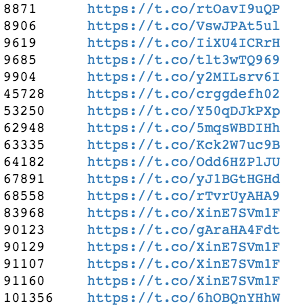
\includegraphics[width=0.5\textwidth]{Cap5/imagens/links}}
	\vspace{0.1cm}
	\caption{Exemplo de \textit{links} extraídos de \textit{tweets}}
	\fonte{Elaborado pelo autor}
	\label{links}
\end{figure}


\lstinputlisting[language=Python, label=extract-link, caption=Extração de \textit{links} provenientes de \textit{tweets}]{Cap5/src/extract-link.py}

Semelhante ao Código~\ref{cod-hash}, é possível aplicar o filtro das \textit{hashtags} para encontrar nomes com maior popularidade através do Código~\ref{cod-fig-pol}. Como pode ser observado nas linhas 8 até 14, em que os nomes dos principais personagens do momento político nacional eram citados.

\lstinputlisting[language=Python, label=cod-fig-pol, caption=Filtro para coletar nomes com mais \textit{tweets}]{Cap5/src/figuras-pol.py}

A partir da linha 16 do Código~\ref{cod-fig-pol} é implementado as informações para a apresentação de um gráfico em setores para a melhor interpretação dos resultados.

Através da utilização do \textit{DataFrame} com a variável "tweets", é possível ainda extrair algumas outras entidades dos \textit{tweets} como a data de criação, nome de usuário, quantidade de seguidores do usuário que publicou o \textit{tweet}, número de \textit{retweets} daquela publicação entre outros. O Código~\ref{dframe} apresenta alguma dessas formas de mapeamento e, também, imprime o número de \textit{tweets} originais e o número de \textit{retweets} que representam a totalidade das publicações coletadas.

\lstinputlisting[language=Python, label=dframe, caption=Extração de outras entidades dos \textit{tweets}]{Cap5/src/dframe.py}

O Código~\ref{category} aproveita o mapeamento das entidades e define uma função para gerar um gráfico em barras que representa o número de \textit{tweets} que alguns usuários realizaram dentro da \textit{hashtag} utilizada para a coleta de dados, ou seja, a \textit{hashtag} \#ImpeachmentDay.

\lstinputlisting[language=Python, label=category, caption=Filtro de usuários através de categorias de entidades]{Cap5/src/category.py}

Uma outra maneira de apresentar os dados coletados foi através do \textit{Word Cloud} ou nuvem de palavras. O Código~\ref{wordcloud} apresenta o desenvolvimento de uma \textit{Word Cloud}, onde contabilizou-se o número de aparições de todas as palavras do conteúdo de texto publicado na rede social \textit{Twitter}.

Para gerar uma \textit{Word Cloud} foi necessário realizar um laço de repetição, conforme demonstrado na linha 3, que verificou cada palavra e removeu algumas exceções, por exemplo palavras iniciadas com "@" \space ou com "RT" \space em seu conteúdo.

A linha 12 apresenta o uso da biblioteca \textit{nltk} para definir algumas palavras que foram bloqueadas como padrão, por exemplo, artigos definidos e indefinidos, que não são necessários a sua contabilização.

\lstinputlisting[language=Python, label=wordcloud, caption=Implementação da \textit{Word Cloud}]{Cap5/src/wordcloud.py}

É possível também utilizar a entidade de localização, apresentada pela API do \textit{Twitter} como \textit{coordinates}, para conseguir as coordenadas de alguns \textit{tweets} e posicioná-las em ambientes de geolocalização possibilitando a criação de um mapa que mostra de qual localidade os \textit{tweets} foram postado, situação esta que permite ao pesquisador verificar qual o estado, região ou país esteve mais ativo durante a coleta da dados.

O Código~\ref{mapa} apresenta o desenvolvimento para este tipo de funcionalidade utilizando a biblioteca \textit{Folium}. No entanto, a forma como o \textit{Twitter} disponibiliza os dados de posicionamento não fornecia a correta localização da postagem. Para tanto, foi necessário inverter a ordem de latitude e longitude disponibilizada pelo \textit{Twitter} para aplicar a correta localização no mapa, conforme apresentado na linha 3.

\lstinputlisting[language=Python, label=mapa, caption=Implementação de coordenadas dos \textit{tweets}]{Cap5/src/mapa.py}

A data de publicação dos \textit{tweets} é identificado pelo atributo "created\_at", onde, através do Código~\ref{time} é possível contabilizar o número de \textit{tweets} de um determinado horário e apresentá-los através de um gráfico.

Por padrão, a API do \textit{Twitter} define o horário de criação dos \textit{tweets} em relação ao Tempo Universal Coordenado (UTC) \cite{twitter-doc}. Logo, foi necessário realizar a conversão para contemplar o fuso horário brasileiro. As linhas 4 e 5 especificam as informações do fuso horário, sendo preciso definir, primeiramente, o horário de \textit{Greenwich} (GMT) e, então, subtrair três horas para considerar o horário de Brasília.

A linha 7 é especificado a contabilização dentro de um intervalo de uma hora e as linhas do Código~\ref{time} que se seguem são as funcionalidades para a criação do gráfico.

\lstinputlisting[language=Python, label=time, caption=Data da publicação dos \textit{tweets}]{Cap5/src/time.py}

Todos os códigos implementados neste trabalho, exceto o Código~\ref{coleta-script} e os \textit{scripts} para a limpeza de \textit{dirty data}, utilizaram a funcionalidade \textit{notebook} do \textit{IPython}para serem implementados, onde foi possível apresentar os códigos ao interpretador do Python utilizando um navegador \textit{web}.

Os resultados apresentados durante a implementação são apresentados no capítulo posterior a este, onde serão analisado os resultados encontrados.




























